\chapter{Conclusion}
This thesis tested and analysed a fully convolutional network (FCN) for segmenting facial images under occlusion. The used network was trained by Nirkin et al \cite{nirkin2018_faceswap} on a rich and diverse dataset. They claim that the speed and the accuracy of this segmentation method outperforms other approaches that were made especially for this task.\\
\\
We evaluated the segmentation accuracy of the network on two real-life datasets. In one of them, every image was supplied with the ground truth labels, which determine whether a pixel belongs to the face or not. A comparison of both segmentations showed that the segmentation of the FCN contained very few false positives. However, the FCN only recognises about 4/5 of the actual facial region (false negatives). In a further step, the network was evaluated on synthetic images in order to be
in full control of all parameters and to be able to simulate every possible face. The results show that there is a hierarchy among the rotations that determine the orientation of the face. Regardless of whether the face is hidden or not, the FCN is the most vulnerable to large roll rotations, then pitch rotations, and least important are the yaw rotations. That is a strange result because no matter how the face is rolled, the information does not change. We expect that the reason for this is the training of the FCN. 

\begin{figure}
	\centering
	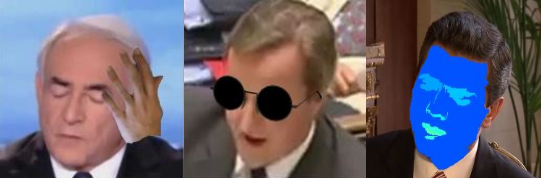
\includegraphics[width=0.5\textwidth]{Figures/chap5/tran_frames.png}
	\caption{Three examples of training images used by Nirkin et al. These are pictures of the recent Janus CS2 dataset by Klare et al \cite{IARPAJanus}. It looks as if the face had not been turned on any of the images in the whole dataset. The first two images are overlaid with synthetic occlusions. The third one depicts the interface used for semi-supervised labeling.}
	\label{fig:chap5:train_images}
\end{figure}

Egger et al \cite{egger_paper} propose an EM-like method to simultaneously segment a face out of a given image and reconstruct it.
We compare the segmentations of Egger et al with the segmentations of the FCN and find that: [1] The approach of Egger et al oversegments the image. [2] The method of Egger et al tends to exclude important details like the eyes due to their strong variability in color and shape. [3] The FCN often fails in recognising and segmenting thin occlusions which is possible with the approach of Egger et al.\\
\\
The runtime of the FCN is much faster compared with the iterative segmentation of Egger et al. On our GPU, the segmentation with the FCN takes approximately 3 seconds, while the algorithm of Egger et al takes 2 minutes (according to the paper \cite{egger_paper} of Egger et al).

\begin{figure}
\centering
\subbottom[original]{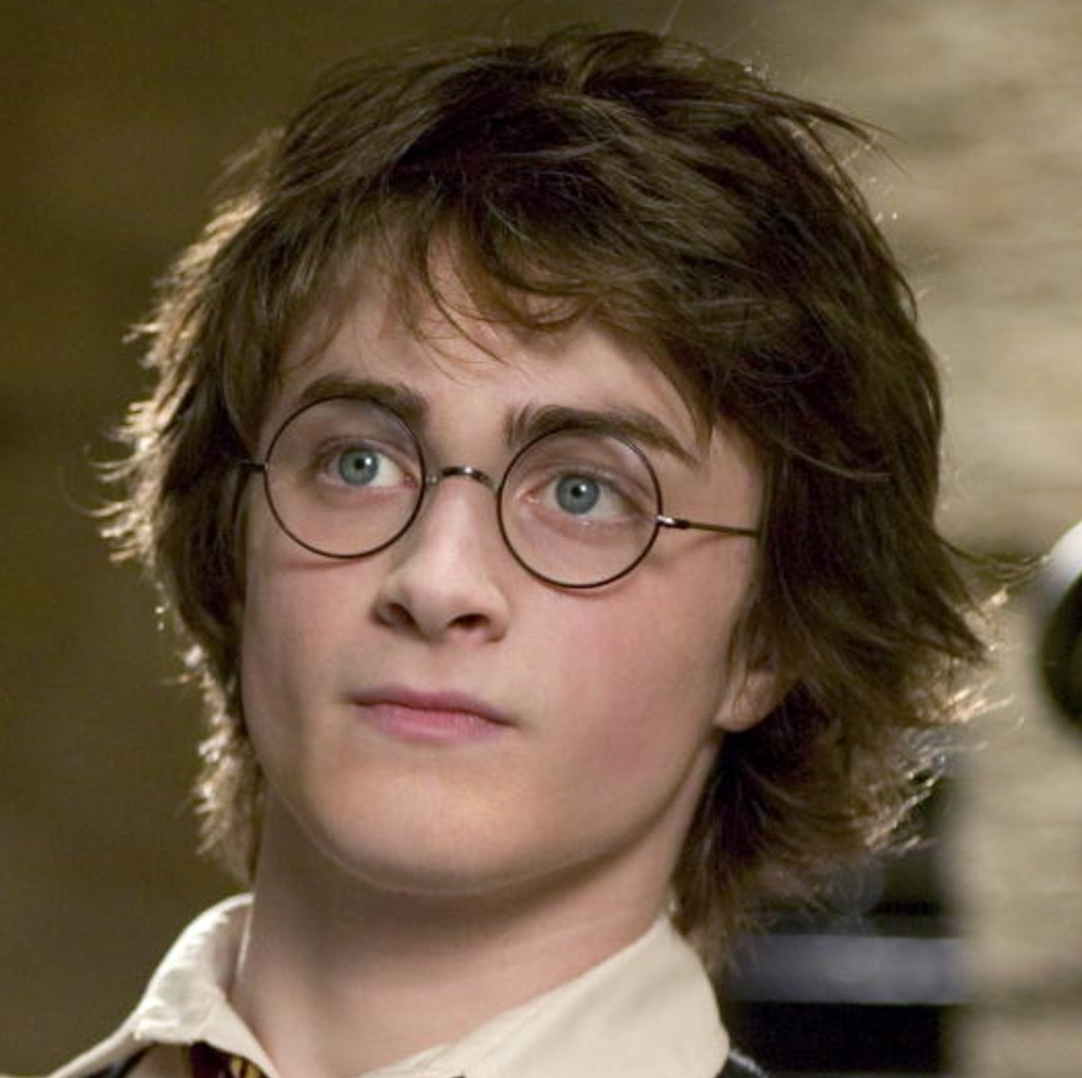
\includegraphics[width=0.2\textwidth]{Figures/chap5/harry_original.png}\label{fig:tm:tm1}}
\subbottom[segmentation of Egger et al]{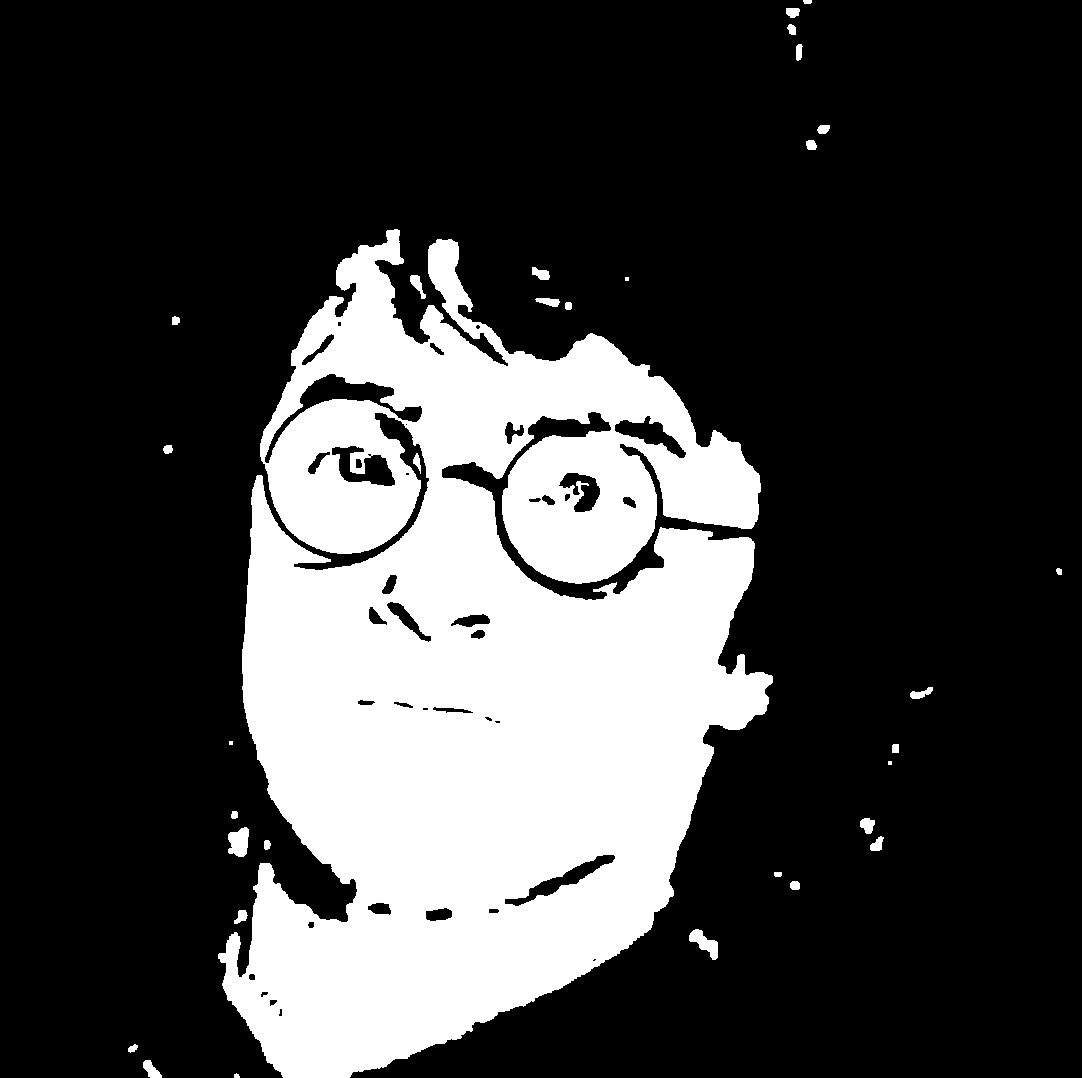
\includegraphics[width=0.2\textwidth]{Figures/chap4/harry_mask_EGGER_.png}\label{fig:tm:tm2}}
\subbottom[segmentation of FCN]{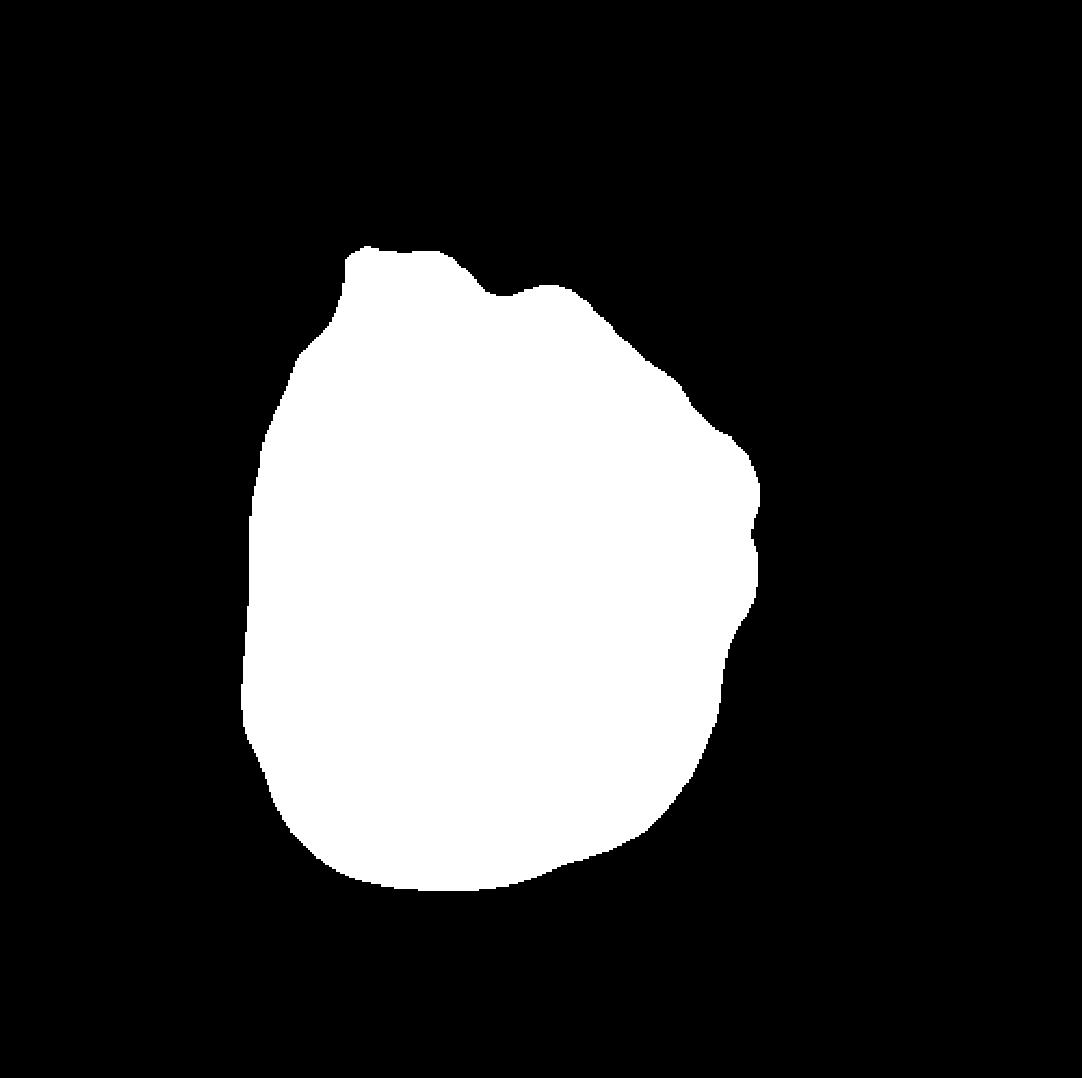
\includegraphics[width=0.2\textwidth]{Figures/chap4/harry_mask_FCN_.png}\label{fig:tm:tm3}}
\caption{Comparison of the two segmentations ((b) and (c)) of the same facial image (a).}
\label{fig:chap5:harry}
\end{figure}

It is difficult to say which mask is better. In order to compare these masks in numbers, both segmentations are used as a mask for fitting synthetic face images, of which we know the correct 3DMM parameters. It turns out that due to the very few false positives of the FCN segmentation, the fit in many cases gets better (in 3DMM parameters) than that with the mask of Egger et al. On the other hand, real facial images are obscured by a variety of objects (not just microphones, hands, and glasses). The method of Egger can recognise these and therefore their mask often leads to better fits on real-world data than with the mask of the FCN [\Cref{appendix:real-world data}].

%Both approaches have their weaknesses and strengths, which we try to combine. Therefore, we take the iterative algorithm of Egger et al and give it the FCN-Segmentation as an initial segmentation. Since this algorithm uses a Metropolis-Hastings method, the final mask looks very similar to Egger et al's mask without the integration.

\section{Future Work}
The Integration in Chapter 4 was not optimal, because the resulting mask came very close to the one estimated by Egger et al itself. Our setting executed the FCN and then let the combined segmentation and fitting algorithm update the mask in all 20 iterations. It would be interesting to see what happens if the algorithm of Egger et al could only improve the initial FCN-Segmentation in a few last iterations. It is strange that the illumination estimation does not improve although an initial segmentation is used for this task (the original approach of egger et al does not use a mask/segmentation to determine the illumination parameters). This is an interesting starting point for further research on how to optimally combine both segmentations.